% ----------------------------------------------------------------
% Report Class (This is a LaTeX2e document)  *********************
% ----------------------------------------------------------------
% ACS 322/420 Dissertation Template
% March 2013, JL

\documentclass[12pt,a4paper]{report}
\usepackage[lmargin=3.81cm,tmargin=2.54cm,rmargin=2.54cm,bmargin=2.52cm]{geometry}
\linespread{1.5}
% Fonts -- the following two packages give your Times Roman in LaTex
%\usepackage{txfonts}
\usepackage{mathptmx}
\usepackage{mathtools} %argmin
\usepackage{verbatim} 
\usepackage{algorithmic}
\usepackage{relsize}

\usepackage{graphicx}
\usepackage{subcaption}
%\usepackage[nottoc]{tocbibind} 
\usepackage{apacite}
%\graphicspath{ {/Users/PureMac/Desktop/Learning_Analytics/Figs/} }
\graphicspath{ {Figs/} }

\begin{document}

\pagenumbering{Roman}

\newpage \section*{ABSTRACT}

% This section is compulsory -- guidelines can be found in the presentation about writing the dissertation.

\newpage \section*{ACKNOWLEDGEMENTS}


%%% Table of Contents

\tableofcontents

\thispagestyle{empty}


% ======================================================== %
%		1. Introduction
% ======================================================== %
\chapter{Introduction}

\pagenumbering{arabic}
\setcounter{page}{1}

% ======================================= %
%		1.1 Background and Motivation
% ======================================= %
\section{Background and Motivation}

% Conditioning paradigms reflects the "neurobiological basis of learning and memory" (Gallistel 2004).  
Learning curves may reflect different underlying learning processes. For example, in insight learning, it may follow slightly fluctuated level and sudden dramatic increase at some points. Because the learning is sometimes the result of experience through personal interactions with the environment. And following the occurrence of insight, abrupt realisation of how to solve the problem can be repeated in future similar situations. This means that the associated experiences with insights can be parameterised, and it can be linked to future behaviours.
% Also, experiences and insight may reinforce each other and can be associated to one another. This associated experience can be memorised and be a feedback as a parameter for future learning. 
% Eventually, behaviour can memorise stimuli and feedbacks, and these may affect and eventually change behaviour.
% insight learning, associative learning, multi-component/process learning.

% These learning processes are reinforced by the conditioned stimulus
% Insight learning is the first cognitive learning.  
% https://psychlopedia.wikispaces.com/insight+learning

%Associative learning : a learning principle that states ideas and experiences reinforce each other and can be mentally linked to one another. Conditioning; behaviour can be modified or learned based on a stimulus and a response. Reinforcers; stimuli used to change behaviour.

Therefore, there are several possible functions which might fit learning curves and represent different learning processes; step function, powerlaw, piecewise powerlaw and etc. Through possible functions and learning curves, people can be grouped into several learning patterns. Moreover, by inspecting people in those groups, 'how they practice' to get the learning curve and 'which features' having an affect upon individuals can be found. Then suggestions for better learning for individuals may be categorised and proposed.

% By fitting those functions to the big data of individuals' game result with various features,
% may influence the individuals' learning curve' 
% on their learning process'

For this, online games are a reasonable instrument. As it involves "rapid perception, decision making, and motor responding", as well as it gives rich details of practice history, in order to find individuals' learning curve and investigate their features (Stafford and Dewar, 2013) 

%\textit{An online game involving rapid perception, decision making, and motor responding. Use of game data-> rich details of training history with measures of performance. Relations between \textbf{practice amount} and \textbf{subsequent performance}, and between \textbf{practice spacing} and \textbf{subsequent performance.}\\
%Greater initial variation in performance is linked to higher subsequent performance-> \textbf{a result we link to the exploration/exploitation trade-off from the computational framework of reinforcement learning.}//
%Explaining two dilemmas: \\
%Reinforcement learning, exploration/exploitation dilemma}

% \subsection{[level 3 heading]}

% As a general rule don't use more than three levels for a heading

Text...

% ======================================= %
%		1.2. Problem Definition
% ======================================= %

\section{Problem Definition}

There are three main issues in traditional reinforcement learning curve. Because it has smooth power law with diminishing gain derived from average value, all possible individual learning curve are squashed into one learning curve. Thus, it cannot tell which learning curve will belong to a task, behaviour, and learning process. Furthermore, even though identifying bad or good on learnings are important, but it cannot provide sufficient information about those.

Below is the list of problems on current reinforcement learning curve.

\begin{itemize}
\item Not being able to categorise learning process.
\item Averaging possible individual learning curves
\item Not enough information for identification of learning success
\end{itemize}
%Explaining about the problem of bootstrapping analysis.\\
%https://en.wikipedia.org/wiki/Bootstrapping (statistics)\\
% "Unless one is reasonably sure that the underlying distribution is not heavy tailed, one should hesitate to use the naive bootstrap"\\
%Bootstrap of the mean in the infinite variance case Athreya, K.B. Ann Stats vol 15 (2) 1987 724-731\\

%%%%%%%%%%%%%%%%%%%
% Piecewise powerlaw? ????? ??? ???? ??? curve? ?? ???? 
% ??? ? ????!
%%%%%%%%%%%%%%%%%%%

% This is a suggested section heading

% ======================================= %
%		1.3. Aims and Objectives
% ======================================= %

\section{Aims and Objectives}
%%%%%
These are the concepts I think you should cover in your introduction:

Skill acquisition \& expertise
- factors which are known to influence skill acquisition
- practice amount, practice spacing, others

Using games to study skill acquisition

Learning curves
- different possible underlying functions
- problems with averaging over

The ultimate aim, of course, is to identify individuals who learn faster or for longer, and try and relate this to how they practice
%%%%%
The aim of this paper is to fit different functions to the Axon game data. In the data, there are 854,064 individuals data about when, where they did the game and other informations, as well as scores of game according to their attempts. And so identify the underlying learning process. Furthermore, it is to inspect features which may have influences on the learning curves. 

\begin{itemize}
\item Understand several possible functions; step function, powerlaw, piecewise powerlaw and etc.
\item Understand different underlying learning processes; insight learning, associative learning, multi-component/process learning and etc.
\item Fit functions to individual Axon game data and compare those to identify.
\item Test theories of what makes learning most effective, exploiting unsupervised learning, establish which parameter is important for getting learning curve from the data.
\item Design more effective learning practices.
\end{itemize}
% This section is compulsory -- guidelines can be found in the presentation about writing the dissertation

%The aim(s) should provide a general idea of what the project is about and the objectives should be more specific. The objectives should be actions that you expect to do (e.g. simulate..., test..., compare...). At the end of the project it should be possible to assess which of the objectives have been achieved. The objectives will also link into the work programme (below).

% ======================================= %
%		1.4. Project Management
% ======================================= %

\section{Project Management}

% This section is compulsory -- guidelines can be found in the presentation about writing the dissertation

Text...

% ======================================================== %
%		2. Data Curation
% ======================================================== %


\chapter{Data Curation}
A large number of data were acquired through the online game named Axon which is developed by Preload for Welcome trust \cite{stuart2009Axon}. In total 1,201,516 machine identities (or players) played the game over 4 million times. The raw data set is fundamentally comprised by the score, date, time of plays and so on in accordance with machine identities which may represent each individual. %\cite{stafford2014tracing}. 
Undoubtedly, it can be possible to extract information from the data set on how people practised to get a higher score. For example, it shows how much time they played for each score. 
However, the raw data set of on-line game seems quite noisy to discern those factors which affect player's learning. It contained many 'undefined' or 'unrepresentable values', and some values are not valid, such as the starting play time is later than the time play finished. For this reason, the information on what the analysis needs cannot be identified directly from it.

Thus, the data source needs refining processes until the gemstone of data set could gleam with the evidence of valuable information. In other words, the big data set has to be curated. Stonebraker et al. stated that "data curation is the act of discovering a data source(s) of interest, cleaning and transforming the new data, semantically integrating it with other local data sources, and deduplicating the resulting composite" \cite{stonebraker2013data}.

\bigskip
Below are the tasks in which steps of data curation are largely expected,

% that this dissertation is interested in, and especially where
\begin{enumerate}
	\item Cleaning raw data set,
	%\item Grouping filtered data set according to the same machine ID,
	\item Incrementally accommodating new data entities,
	\item Normalising scores grouped by the same players,
	\item Clustering players, showing the similar patterns.
\end{enumerate}

In particular, data curation tasks followed methods of two previous studies
\cite{stafford2014tracing, stafford2016testing}.
Accordingly, the curation tasks of cleaning, grouping by machine IDs and accommodating will be explained in the following section. After that, other tasks for data deformation and clustering will be examined.

\begin{comment}
which certified "the relationship between the practice amount and subsequent performance, and between practice spacing and subsequent performance" and "the consolidation effect for skill learning". In order for these analyses, unnecessary information contained in the data set had to be filtered, and additionally, the new variables were augmented by manifesting some hidden features in the same player through those two analyses.

In gratitude, filtering methods on the data source was already regularized in some degree by Stafford et al. (2014; 2016).
\end{comment}
% , K-Means clustering, with the artificial neural network algorithm, competitive learning 

% ======================================= %
%		2.1. Data Cleaning
% ======================================= %
\section{Data Cleaning}

What has to be noted before data cleaning is that it has to be implemented under the grouped data by the same machine IDs. In toal 4,038,802 plays were sorted by players having the same machine IDs, and then 1,201,516 players were detected. The criteria according to the previous two studies \cite{stafford2014tracing, stafford2016testing} are as follow,
% Though the two studies in 2014 and 2016 about skill learning analysis using the game data source, some curation steps were performed by the following criteria.

%\begin{itemize}
%	\item 26,727 players who did not play a minimum of 15 games were eliminated,
%	\item 8\% out of the total number of players attempted more than 300 times, and those were also discharged.
%	\item 26,175 data which lack valid longitude or timing information for each attempt were filtered.
%\end{itemize}

\begin{enumerate}
	\item players who did not play at least 15 games,
	\item players who attempted more than 300 times,
	\item data which lack valid longitude or timing information for each attempt,
	\item players with discontinuous game play attempts.
\end{enumerate}

The reason of discarding those who played less than 15 attempts is because those cannot show a causal relationship between attempts and scores. In this step, xxx individuals were deleted. 
The reason for second step is that plays more than 300 attempts did not show many differences after 300 attempts. ??? out of the total number of players attempted the game more than 300 times, and also they were removed. Also discarded players having unrecognisable time information were ???. Finally, game play data for individuals were recorded discontinuously. In other words, there are non-recorded game play data between the first attempt and the last attempt for each players. The reason why this problem happened is unknown, though it is obvious that individuals with this issue have to be filtered appropriately. Though cleaning those is simply mentioned in this session, the specific method how to manage players with discontinuous data will be discussed in chapter ???.

As a result, raw data with 4, 038,802 plays with xxx players were cleaned, and then reduced to ??? plays and ??? individuals decreased by ???.

\section{Data accommodating}
The next step of data curation is to incrementally accommodate hidden but obvious features from the previous cleaned data set. It is originally constituted by 8 basic categories. After data accommodating task, 7 additional hidden variables would be derived.

\subsection{Original variables in the data source}
When people play the on-line game, 7 basic features as follow is recorded,
\begin{itemize}
    \item machine identities,
	\item scores and attempt numbers,
	\item date, hour and minute,
	\item latitude and longitude.
\end{itemize}

When players access the on-line game, the tracking code written by Preloaded records machine identities. Machine IDs may be considered as individuals who actually play the game. Preloaded inserted tracking code to the on-line game, records a machine identity at each time the game was loaded, as well as the result of the game at the end of plays, and play date and time. Attempts and scores were recorded in the order of the time.

The information of locations where the machine ID accessed the game is also collected approximately at the maximum of city-block level.

\subsection{Hidden variables calculated from the original variables}
From the basic variables which are recorded when people play the game, other features that may imply useful information of how players are influenced during learning processes to get higher marks can be derived as below,

\begin{itemize}
	\item time difference,
	\item local time,
	\item gap types (no, long, short and sleep gap),
	\item a number of total plays.
\end{itemize}

The basic time information; date, hour and minute is combined together. Then, time differences between successive attempts are calculated by subtracting current game start time from its previous attempt time. Therefore, the first attempts do not have value of time differences.

\bigskip
Next, local times for each play were calculated in seconds, using the formula, "$\textit{local time} = \textit{UTCtime} + (\textit{longitude} � 24\div360),\textit{modulo}24$" \cite{stafford2016testing}. Local time would facilitate comparison of players in different time zones, thus indicating lifestyle choices. There were data that local time could not be calculated because of missing track of latitude and longitude, and those were filtered at the data cleaning task.

\bigskip
On the basis of time difference, Stafford et al. (2016) classified individuals into 4 groups, according to "the nature of the timing of their first 15 attempts at the game". First group is 'no gap' for those who had less than 15 minute break between each play. Second group is 'wake' in which players are assumed to be having a rest in their waking hours if they have "a single gap between 7 and 12 hours". Working hours is time between 5 am and 12 pm. Those who rested for between 7 and 12 hours in working hours were categorised as 'sleep'. Finally, all other individuals are classified as 'no category'.

Furthermore, for more detailed analysis, 'rest' which is defined in 'gap types' categorisation was divided with 3 types. Long gap, short gap and sleep gap were determined when players had a rest 'between 7 hours and 11 hours', 'below 15 minutes', and 'not in working hours' respectively.

\bigskip
As the term of hidden variables suggests, there are possibilities that more factors can be mined from the data set and be incrementally accommodated to it if appropriate methods are implemented.

\section{Data Deformation}
CSV format has been used as a basic data file format for previous study.

CSV is an abbreviation of Comma-Separated Values. A data record of CSV format file is a line formed by one or more elements, and commas separate those element values to be distinguishable (plain text format) \cite{shafranovich2008common}. According to Idris (2014), it is straightforward for those format to load and store data-set from the data storage onto working place; ease to generate, read and edit manually, offer versatility in most programming languages, but not efficient because exploiting plain text format "take a lot of space". This might result in consuming more time to handle such a big data set than using binary format.

Simply, the data set needs to be stored in memory unit of machine(s) where the analysis processes would operate. However, these are true only when data size is manageable. Because fitting all data-set of such a large amount of data in computer memory takes many spaces. In some cases, loading on computer memory cannot be possible depending on computer capability and setup. Thus, CSV format is not a very efficient way to manage such a large amount of data \cite{idris2014python}. To solve those problems, two approaches of being able to reduce storing spaces and of enabling faster speed for analysing were applied; converting CSV file format into Pickle format, and splitting data set into several pieces.

\subsection{Pickle file format}
Pickle file format can provide "a high level of data compression such as zip, bzip and gzip" and also faster than CSV \cite{idris2014python}, because it is "binary protocols for serializing and de-serializing a Python object structure" \cite{python2016pickle}. Furthermore, it provides on easy approach to deal with converting Python object hierarchy into a binary stream and vice versa, with the notion of 'pickling' and 'unpickling'. Moreover, pickle file format can automatically represent a large number of Python types \cite{python2016pickle}.

\bigskip
Therefore, curated data set after cleaning, accommodating, and deformation process is stored as binary file format, and for the binary file format, pickle specified for Python is used.

\subsection{Data storage and index table}
Although the big data set can be converted to binary file, it still takes a large amount of storage. And it also causes RAM memory optimisation problem. When data curation tasks are performed (of course, as well as data analysis tasks which will be discussed in the next session), processing speed became slower and slower over time. This might be because data occupies all spaces of hardware memory, and exploits virtual memory on main memory unit. Basically, RAM memory provides very high speed compared to hard disk, and it is even faster than Solid State Drive (SSD) which is often considered 'fast'. If data take all RAM memory spaces, they transfer addresses of some part of it to virtual memory. This task causes many interruptions to the tasks, and eventually decreases processing performance significantly. And depending on operating systems, Python kernel may crash.

\bigskip
Therefore, loading only necessary data to a specific task will be a solution to keep processing performance fast. Whole data set was separated by each type of variables. To secure and not to lose player information within the divided data, addresses of all data have to be indexed directing player ID. As a result of data deformation task, 15 pickle data files were generated; eventLabel, date, hour, minute, latitude, longitude, eventValue, play\_filter, comb\_time, diff\_time, local\_time, long\_gap, shor\_gap, sleep\_gap, gap\_type, and total\_plays, which are indicated by individual ID information, eventAction.

%%%%%% comment %%%%%%%%%%%%%
\begin{comment}
(Python 2001)
There are various file formats which can provide a high level of data compression.

, which is formed from 15 factors, into the data vector having like hash table

By default, the pickle data format uses a relatively compact binary representation. If you need optimal size characteristics, you can efficiently compress pickled data.


?CSV is human readable and easy to edit manually
?CSV is simple to implement and parse
?CSV is processed by almost all existing applications
?CSV provides a straightforward information schema 
?CSV is faster to handle
?CSV is smaller in size
?CSV is considered to be standard format
?CSV is compact. For XML you start tag and end tag for each column in each row. In CSV you write the column headers only once.
?CSV is easy to generate

Since, depending on your computer setup you might not be able to fit it all in memory, we'll load each class into a separate data-set, store them on disk and curate them independently. Later we'll merge them into a single data-set of manageable size.
\end{comment}

% ======================================= %
%		2.4. K-Means Clustering with Competitive Learning Algorithm
% ======================================= %
\section{K-Means Clustering with Competitive Learning Algorithm}

In order to identify learning curves of individuals, the first thing to do is to cluster players into several groups in which they show similar learning patterns. Traditional ways of identifying individual learning curves is either averaging all data of test subjects or fitting different possible underlying functions to observed population data-set \cite{newell1981mechanisms, gallistel2004learning, donner2015piecewise}

\bigskip
A well represented learning curve in psychology might be a "smooth power law of diminishing gains" \cite{donner2015piecewise}. For example, Howard (2014) tested function fitting on chess performance and verified that "power function fit is best". 

However, in contrast, Gaschler et al. (2014) stated that "the exponential function" is "better than the power function fitting" for learning curves of chess players. These different results of the same observation of chess game would result from that the power law is an artifact which averages many divergent shapes of exponential curves (Heathcote et al., 2000; Murre \& Chessa, 2011) as well as other possible underlying curves. 

Therefore, before analysing the on-line game data set, it would be a better assumption that there are many different shapes of learning curves depicting individuals' learning best, rather than only one learning curve. 
% Hence, it would be better to cluster players by similar learning patterns before identifying which curve functions will fit best on the on-line game data-set.

\bigskip
In contrast with classification tasks that classify labelled data-set, clustering is an unsupervised classification task which automatically groups similar data without predefined and labelled classes \cite{hackeling2014mastering}, and it generates the same result as classification algorithm does \cite{harrington2012machine}. 

Among several clustering methods, K-Means clustering was used with an artificial neural network algorithm, competitive learning.
%, for the analysis of the on-line game data set. 
It is because K-Means clustering algorithm in high dimensions is computationally very slow and the key method of K-Means (comparing distance in 2 and 3 dimensions) would not work for satisfying outcome in high dimensions \cite{daume2012course}.

\bigskip
Hence, there is possibility that the data-set may not properly be clustered, as the on-line game data-set is comprised of 15 dimensions. Compensating K-Means clustering with neural network algorithm would provide one of the solutions for the high dimensions data-set.

% ======================================= %
%		2.4.1 K-Means clustering
% ======================================= %
\subsection{K-Means clustering}
The name of K-Means is because it discovers k unique clusters, and the mean values of those clusters represent the centres of each cluster. The key idea of the algorithm is to compare only distances between all data and arbitrary number of cluster centres. After centroids of clusters were found, all data can be assigned to their nearest centres. In the same manner, centres of clusters can be computed after data is allocated to clusters.

Again, there are no labels or predefined information of classes in the data set. %In other word, 
Thus, it is unknown which approach has to be implemented first. The ways to tackle this are to start with initial random point, to iterate calculation of centre position, and to rearrange elements in clusters. Through iterating these three approaches until stopping criteria is satisfied, k means eventually converge to local optimisation, and comprise k number of clusters. 

\bigskip
There are two terminating criteria in K-Means clustering algorithm. The first one is using a threshold for the difference of cost functions (\ref{eq:k_means_cost_function}) through subsequent iterations (\ref{eq:threshold1}).

\begin{equation} \label{eq:threshold1}
	J_i - J_{i-1} < \theta \quad \textrm{, where} \; j \in K,
\end{equation}

and cost function $J$ is

\begin{equation} \label{eq:k_means_cost_function}
    J(\mathbf{\mu, C; D}) = \sum_n^N || x_n -\mu_{C_k} ||^2
    = \sum^K_{k=1} \sum_{i \in C_k} ||x_i - \mu_k||^2,
\end{equation}
where $\mu$ is mean of cluster, $\mathbf{D}$ is \ (the number of parameters) data-set, $\mathbf{C}$ is clusters in the data-set, $x$ is data, $N$ is the number of data, and $K$ is the number of clusters. 

The other one is to use a threshold for the difference of centre positions between successive iterations (\ref{eq:threshold2}).
\begin{equation} \label{eq:threshold2}
    x_i - x_{i-1} < \theta \quad \textrm{, where } i \; \textrm{in} \; C_k \,.
\end{equation}

\bigskip

Below is pseudo-code of K-Means clustering algorithm, 
\bigskip
\begin{algorithmic}
\FORALL{$k$ such that $ 0 \leq k < K$}
	 \STATE randomly initialise $\mu_k$
\ENDFOR
\smallskip
\WHILE{stopping criteria (\ref{eq:threshold1}) or (\ref{eq:threshold2})}
	\FORALL{$k \in K$}
		\FORALL{$i$ such that $ 0 \leq i < N$}
			\STATE $\mathbf{C}_k \leftarrow \underset{x}{\arg\min}|| \mu_k - x_i ||^2$ ,\\
		\ENDFOR
	\ENDFOR
	\smallskip
	\FORALL{$k \in K$}
		\STATE $\mu_k \leftarrow \textrm{mean}(\mathbf{C}_k)$
	\ENDFOR
\ENDWHILE
\RETURN $\mathbf{C, \mu}$
\end{algorithmic}
%After finding centers of clusters, each data are assigned to its nearest clusters.

\bigskip
At first, the positions of centroids are randomly initialised. Then, the first for loop in the while loop assigns each data to nearest clusters. The second for loop calculates the centres of clusters. By iterating these two tasks, all centroid of clusters move slightly towards the centres of each cluster, and eventually converge to local optima. For on-line game data analysis, stopping criterion (\ref{eq:threshold2}) was used. 

Moreover, this K-Means clustering algorithm was improved with artificial neural network, competitive learning algorithm, in order to cluster the on-line game data-set in high dimensions.

% ======================================= %
%		2.4.2 Competitive learning
% ======================================= %
\subsection{Competitive learning}

Competitive learning is unsupervised learning approaches in which the output neurons contend against each other to react as the one firing from the given pattern in inputs. Therefore only one unit take the winner upon all output units (\ref{fig:Competitive_Diagram}). This exclusive phenomenon in synaptic neurons is called 'winner-take-all units', and sometimes they are also called 'grandmother cells'. Which means a neuron fires on a specific stimulus. This neural networks has an advantage of clustering unlabelled data and searching the correlations of the input data. One of the most significant application of competitive learning might be vector quantisation. In which, input data-set becomes a bunch of vectors in data space, and input vectors are compressed and stored by transmitting into prototype vectors.

\begin{figure}[ht]
    \centering
    \framebox{\parbox[t][0.7\textwidth][t]{0.95\textwidth}{
        \begin{center}
            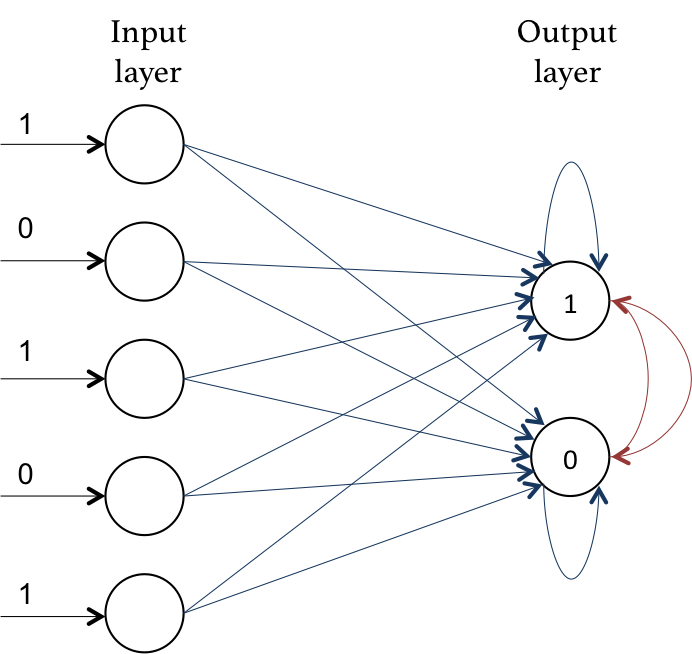
\includegraphics[width=0.85\textwidth, height=0.65\textwidth]{Competitive_Diagram.png}
        \end{center} }}
	\caption{Competitive neuron diagram. When an input enters the network, it generates output values according to weights between an input and output neuron (blue arrows). Output neurons compete with each other (red arrows), then only one output fires on an input pattern. Output neurons are considered only having binary $0/1$ output.}
	\label{fig:Competitive_Diagram}
\end{figure}

\bigskip
It has a very similar concept to K-Means clustering algorithm. The prototype vectors can be interpreted as centroids in k-means. Besides, vector quantisation employs Euclidean metric to assign an input vector to the nearest prototype, weight vector. When input data, usually represented as a vector, are applied at the input of the network, the winner neuron indicates the appropriate class. 

If all input data are entered to the network, the input space organises a Voronoi tessellation. To be specific, Voronoi tessellation which was used for the analysis is Centroid Voronoi tessellation, in which means are positioned in each Voronoi cell (centre of mass). The weight vectors (or centroid in K-Means) are the vectors of prototypes. 

\bigskip
Output neurons $O_i$ in (\ref{eq:competitive1}) are the units having the net input in an pattern at a time,
\begin{equation}\label{eq:competitive1}
    O_i = \sum_j w_{ij}x_j = \vec{\mathbf{w_i}} \cdot \vec{\mathbf{x}},
\end{equation}
for an input vector $\mathbf{x}$. 

Winner neurons are found by (\ref{eq:competitive2}),
\begin{equation} \label{eq:competitive2}
    \vec{\mathbf{w}}_k^T\vec{\mathbf{x}}^\mu > \vec{\mathbf{w}}_i^T\vec{\mathbf{x}}^\mu \quad \textrm{for all i},
\end{equation}
where winner neuron is $\vec{\mathbf{w}}_k^T$, and $\vec{\mathbf{x}}^\mu$ is an input of pattern $\mu$.

\bigskip
(\ref{eq:competitive2}) tells winning unit is the biggest. If the weight vectors connecting between each input and output are normalized, $\vec{\mathbf{w_i}}=1$, then (\ref{eq:competitive1}) can be redefined as below,
\begin{equation} \label{eq:competitive3}
    \quad |\vec{x}^\mu - \vec{w}_k^T| \leq |\vec{x}^\mu - \vec{w}_i^T|, \quad
    \textrm{only if} \;\; |\vec{w}=1| \;\; \textrm{for all i.}
\end{equation}

\bigskip
(\ref{eq:competitive3}) shows similarity to the key idea of K-Means clustering, which only consider distances between all data and centroids.

\bigskip
Competitive learning only consider the output neuron with the maximum net value of inner product between input and weight. Biologically, output neurons are connected with other output neurons with lateral inhibition, as well as excitatory connection itself, and therefore winner takes all units.
%output neurons have a value of $\vec{w}^T\vec{x}^\mu$, thus the largest output is always win. 

\bigskip
For competitive learning, the thing to note is that weights must be normalised in order for all units to have a unit length.

% ======================================= %
%		2.4.3 Normalisation
% ======================================= %
\subsection{Normalisation}
Normalisation is important for analysing data with different scale to be compared and then to derive information in K-Means clustering \cite{bowles2015machine}. To be specific about normalisation for competitive learning, the network exploits the inner product for each input with weight vectors in order to identify winner output unit. If looking inside of (\ref{eq:competitive2}), the equation for inner product is
\begin{equation}\label{eq:inner_product}
    \vec{\mathbf{w}}^T \cdot \vec{\mathbf{x}}^\mu = \vec{\mathbf{w}}^T\vec{\mathbf{x}}^\mu \cos(\theta),
\end{equation}
with respect to the lengths of both units and a direction between input pattern and weight. Not-normalised one has no way for a criterion for competing output units with weight vectors. Because the neuron which has the largest value in length always wins. That implies the algorithm will finish without any learning or no informative outcome through iterations, in the both cases of not-normalised data-set and weight vectors.

\begin{figure}[t]
\begin{subfigure}{0.5\textwidth}
    \centering
    \framebox{\parbox{0.95\textwidth}{
        \begin{center}
            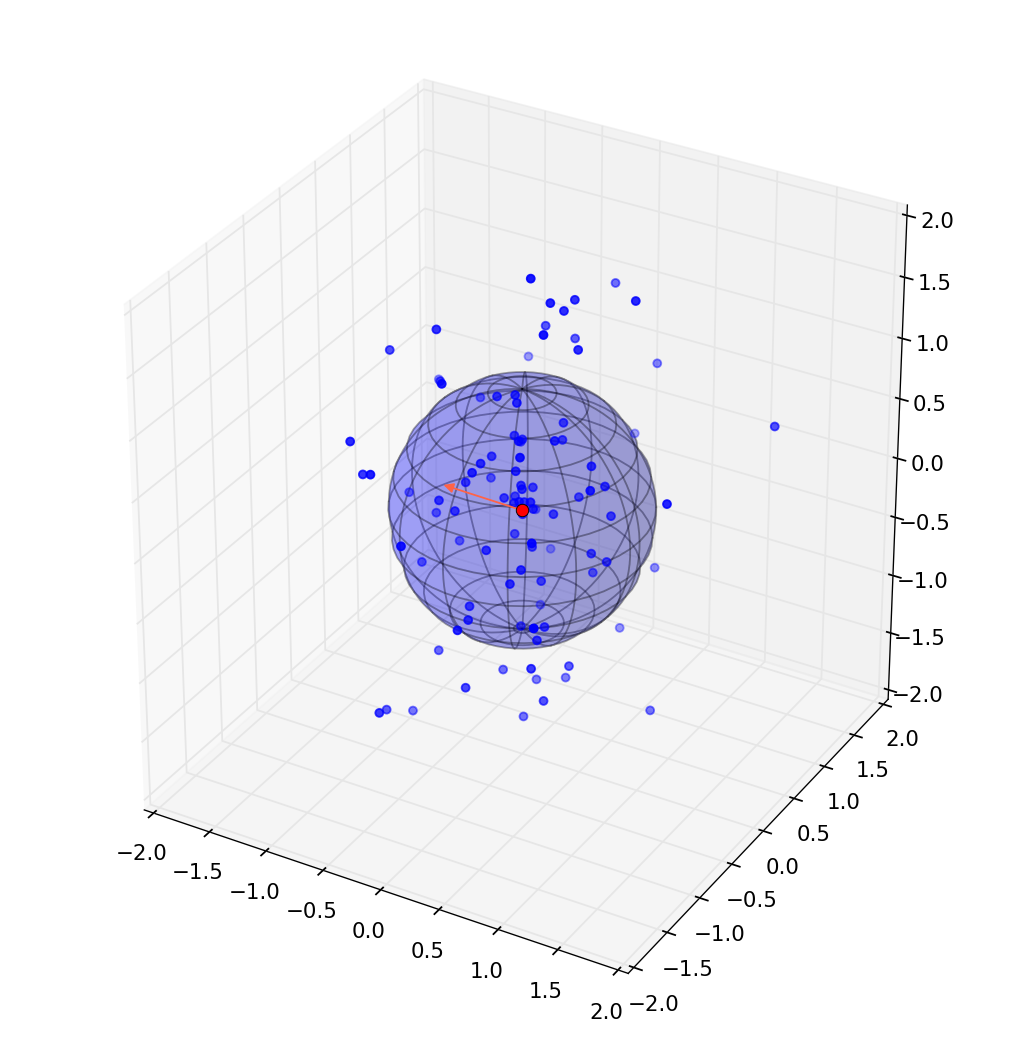
\includegraphics[width=0.9\textwidth, height=0.9\textwidth]{not_norm_data.png}
        \end{center} }}
    \caption{Not-normalised data with a unit weight (red arrow)}
    \label{fig:not_norm_data}
\end{subfigure}
\begin{subfigure}{0.5\textwidth}
    \framebox{\parbox{0.95\textwidth}{
        \begin{center}
            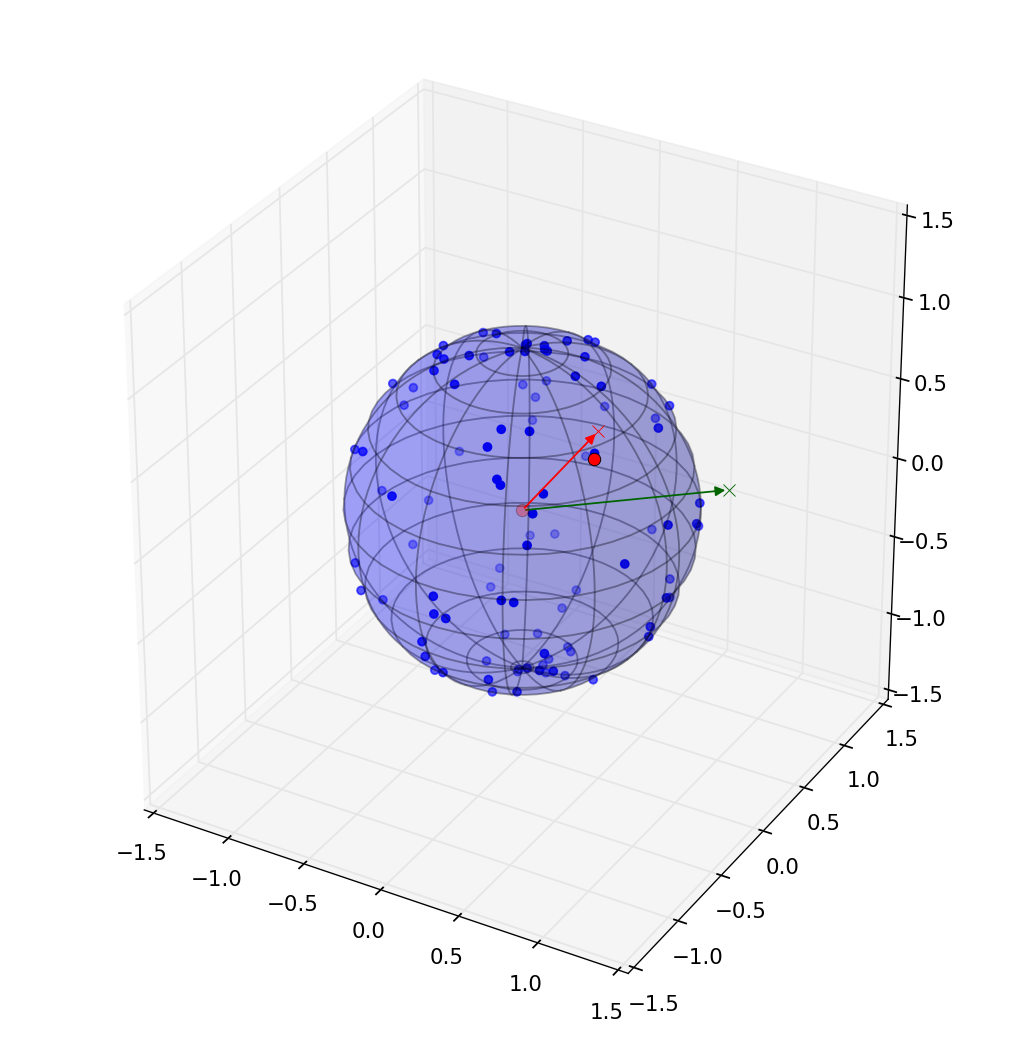
\includegraphics[width=0.9\textwidth, height=0.9\textwidth]{not_norm_weight.png}
        \end{center} }}
    \caption{Normalised data-set with not-normalised weight vectors (green arrow).}
    \label{fig:not_norm_weight}
\end{subfigure}
\caption{Examples of not-normalised data and weight in 3 dimensions. In both left and right figures, sphere represents unit length area.}
\label{fig:not-normalised}
\end{figure}

\bigskip
For the solution of that, normalising input and weight vectors simply transforms (\ref{eq:inner_product}) into the equation computing only a direction between those vectors, which tells how close weight vector is from the input vector. 

Eventually, the inner product in (\ref{eq:competitive3}) becomes the criterion which detects the shortest Euclidean distance by comparing angles between input and weight vectors, (\ref{eq:distance}).

\begin{equation}\label{eq:distance}
    \begin{split}
        \vec{\mathbf{w}}_k^T \cdot \vec{\mathbf{x}}^\mu &> 
        \vec{\mathbf{w}}_i^T \cdot \vec{\mathbf{x}}^\mu \\
        \cos(\theta_k) &\geq \cos(\theta_i).
    \end{split}
\end{equation}

The firing output neuron still has the largest value among output units when the $\theta$ is smaller than others based on the competition with proximity of the input vector.

(\ref{fig:not-normalised}) shows not-normalised issue in competitive learning. In the not-normalised data-set and weight vector, (\ref{eq:inner_product}) always compares only the length, not the closest one in the distance between data and weight vector. It is obvious that the most long vector always win, which cannot be representative for input patters. Thus weights would not move to the centre of Voronoi cell.

% ======================================= %
%		2.4.4 Procedure of the algorithm
% ======================================= %
\subsection{Procedure of the algorithm}
After normalising data-set and setting weight vectors with unit length, the competitive learning algorithm for pattern classifier exploiting (\ref{eq:competitive1}) and (\ref{eq:distance}) follows as below,

\begin{enumerate}
\item {choose weight vector with random values}: \newline
Similar to K-Means clustering, weight vectors which implies center of mass for clusters (or Voronoi cells) are initialised with random values. However, the issue of dead unit would be caused by randomly initialised weight vectors. Dead unit is the unit which is very far from any input patterns, and therefore never fires. An other problem is the optimal number of weight vectors. This problem will be discussed in the next section. The last thing to be noted is that weight vector must have unit length.

\item apply input patterns to the network in turn or in random order: \newline
After setting initial weights, input data vector as a pattern is entered to the network. It does not matter applying it in turn or in random order. The advantage of competitive learning over K-Means is that K-Means comparing all data, then must be slow, but competitive learning can run in random order input data until it approaches the sufficient learning rate. Therefore it is much faster than K-Means, on condition of how learning rate is prescribed.

\item discover a winner output unit for each input: \newline
When an input vector is applied to the network, which output unit is likely to take winner position for each normalised input pattern is found through (\ref{eq:distance}). For a given input pattern, the winner unit has the largest value among other output neurons. In other words, winner-take-all unit is the closest vector to the input vector with the smallest angle. Inhibitory and self-exitatory connection are definded biologically, but alternatively using python command, \textbf{numpy.argmax}, just maximum value is searched.

\item Update the winner neuron's weight to be close to the input vector: \newline
For each input, winner $\mathbf{w_k}$ is found among the outputs, and then it is updated to be closer by an allowed amount with learning factor $\eta$ to the current input vector. After continued update of the weight for the winner unit, weight vectors will be positioned at the center of Vornoi cells which shows similar patterns of inputs. Below is on-line and batch update rule,
	\begin{equation} \label{eq:on-line and batch}
	\begin{split}
	    \text{on-line rule}&: \Delta \vec{w}_k = \eta(\vec{x}^\mu - \vec{w_k})\\
	    \text{batch rule}&:\Delta \vec{w}_k = \eta \Sigma_{\mu \in C_k} (\vec{w_k} - \vec{x}^\mu)
	    %\text{or} \quad \quad \quad&
	\end{split}
	\end{equation}
On-line learning rule updates the change of one data point at a time. However, batch learning rule accumulates weights until all inputs in a cluster are passed to the network, and sums all of those constantly. Both converge the same centroids of clusters, but batch rule is slower than on-line learning rule which slightly fluctuates towards local optima when updating.
\end{enumerate}

As mentioned in procedure 1, choose weight vector with random values, the two possible problems; the number of clusters and dead units, of competitive learning have to be handled with proper method. The next section will introduce breakthroughs which can tackle those two issues.
% ======================================= %
%		2.4.5 Local optima and optimal number of clusters
% ======================================= %
\subsection{Local optima and optimal number of clusters}

Sometimes, a number of mean values might be randomly initialised very nearly to each other. And centroids would converge a same point in a same cluster. In this case, clusters would not describe data-set informatively. This issue is called local optima problem. Unfortunately, there is "no way of knowing what the right answer is" for the outcome of clustering algorithm, but "repeating the algorithm dozens or even more times" can increase reliability of clustering result \cite{hackeling2014mastering}. By repeating clustering algorithm several times, the starting random data points will be set differently and converge different or the same local optima as subsequent outcomes. Clustering results are compared relatively with repeated results, and the most frequent similar results can be presumed as reliable result.

%\begin{figure}[thpb]\label{fig:elbow}
%	\centering
%	\framebox{\parbox{5.5in}{ \includegraphics[scale=0.55]{elbow_method.png} }}
%	\caption{Cost values according to the different number of k}
%\end{figure}

\bigskip
Another crux of K-Means clustering is that the optimal number of clusters is unknown. There are ??? players in the on-line game data-set, and it has no predefined information of how many groups showing what the similar learning patterns are. To estimate optimal number of clusters, Elbow method with Bayes and Akaike Information Criteria (\ref{eq:AICandBIC}) was used. The criteria which can determine the number of cluster is as follow,
\
\begin{equation} \label{eq:AICandBIC}
    \begin{split}
        \textrm{Bayes Information Criteria (BIC)}:&\quad \underset{K}{\arg\min} (J_K + K\log D)\\
        \textrm{Akaike Information Criteria (AIC)}:&\quad \underset{K}{\arg\min} (J_K + 2KD).
    \end{split}
\end{equation}

\bigskip
The more a number of clusters, the less the value of the cost function, $J_K$. Because, increasing K can divide the data-set into smaller pieces of clusters than the actual number of how many clusters necessarily exists in it. Usually, using the Elbow method shows changes of the value of cost function. It goes down significantly at first some K, and suddenly slows down the change. By inspecting the point showing from dramatic to gradual change, generally the optimal number of K is detected. 

However, when only Elbow method for the on-line data-set is plotted, this inflection point is rarely found. Because all costs seem decreasing gradually, Fig.~\ref{fig:AIC_BIC_Elbow}. Therefore, BIC and AIC was exploited with Elbow method. If plotting AIC values in different number of K, it will decrease by the certain amount cost, and then start to increase. It is because $2KD$ or  $K\log D$ proportionally compensates decreasing the value of cost function for various number of K. In high dimensions, AIC criteria gives "high penalty for many clusters" \cite{daume2012course}. As a result, K value which minimizes AIC or BIC (\ref{eq:AICandBIC}) could be considered as the optimal number of clusters. 

\begin{figure}[thpb]
	\centering
	\framebox{\parbox{14cm}{
	    \begin{center}
	    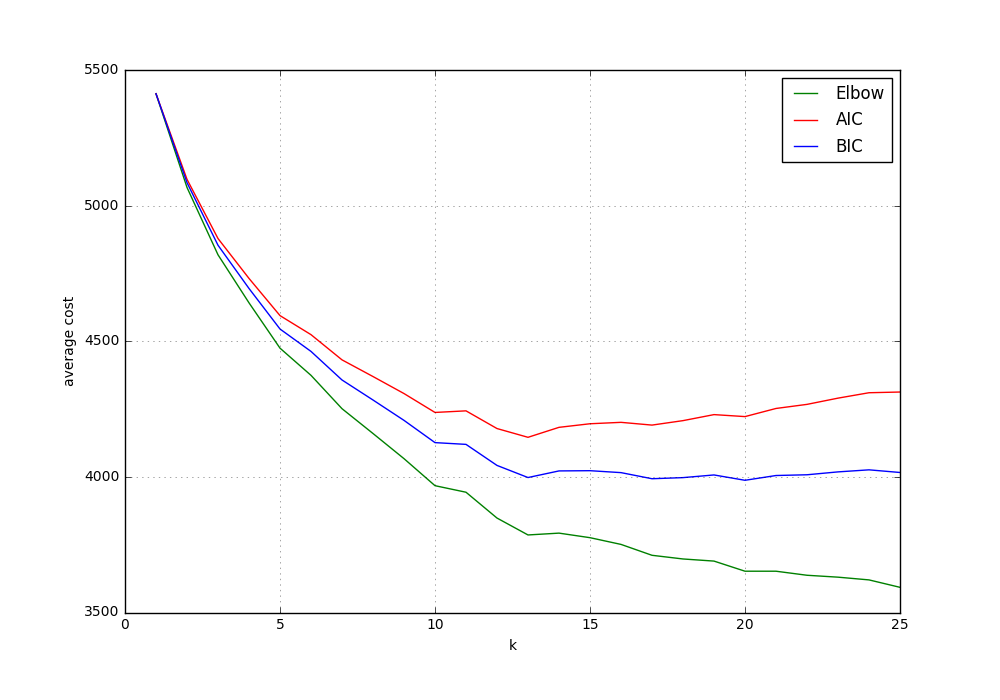
\includegraphics[width=14cm]{AIC_BIC_Elbow.png}
	    \end{center} }}
	\caption{Comparison between AIC and BIC according to the different number of k. AIC are more strict method than BIC to identify the number of clusters.}
	\label{fig:AIC_BIC_Elbow}
\end{figure}

\bigskip
Fig.~\ref{fig:AIC_BIC_Elbow} shows the information of elbow method with AIC and BIC to define the number of clusters for the on-line game data-set. By these three graphs, it seems that the data-set can be clustered into n clusters. Difference between 13K and 14K is xx and, 14 K and 15 K is yy. If the number of 14 is set as a threshold for these differences, increasing K beyond 14 would not improve the result of clustering.

% ======================================= %
%		2.4.5 Dealing with dead unit
% ======================================= %
\subsection{Dealing with dead unit}
A common problem in competitive learning algorithm is dead unit issue. This is the case when weight vectors are initialised far distant from all input vectors. As they cannot fire among those which are closer to input vectors. Geometrically speaking, (\ref{fig:dead_unit}) would show precise understanding. Two arrows with different colours represent randomly initialised weight vectors. Red arrow is closer to two input groups than green weight vector. When they are threw into the network, red weight vector will move closer and closer to the centre between two groups at every iterations. Which means red weight vector always takes winner, and green weight vector will never be updated. 

\begin{figure}[hb]
    \centering
    \framebox{\parbox[t][0.8\textwidth][t]{0.9\textwidth}{
        \begin{center}
            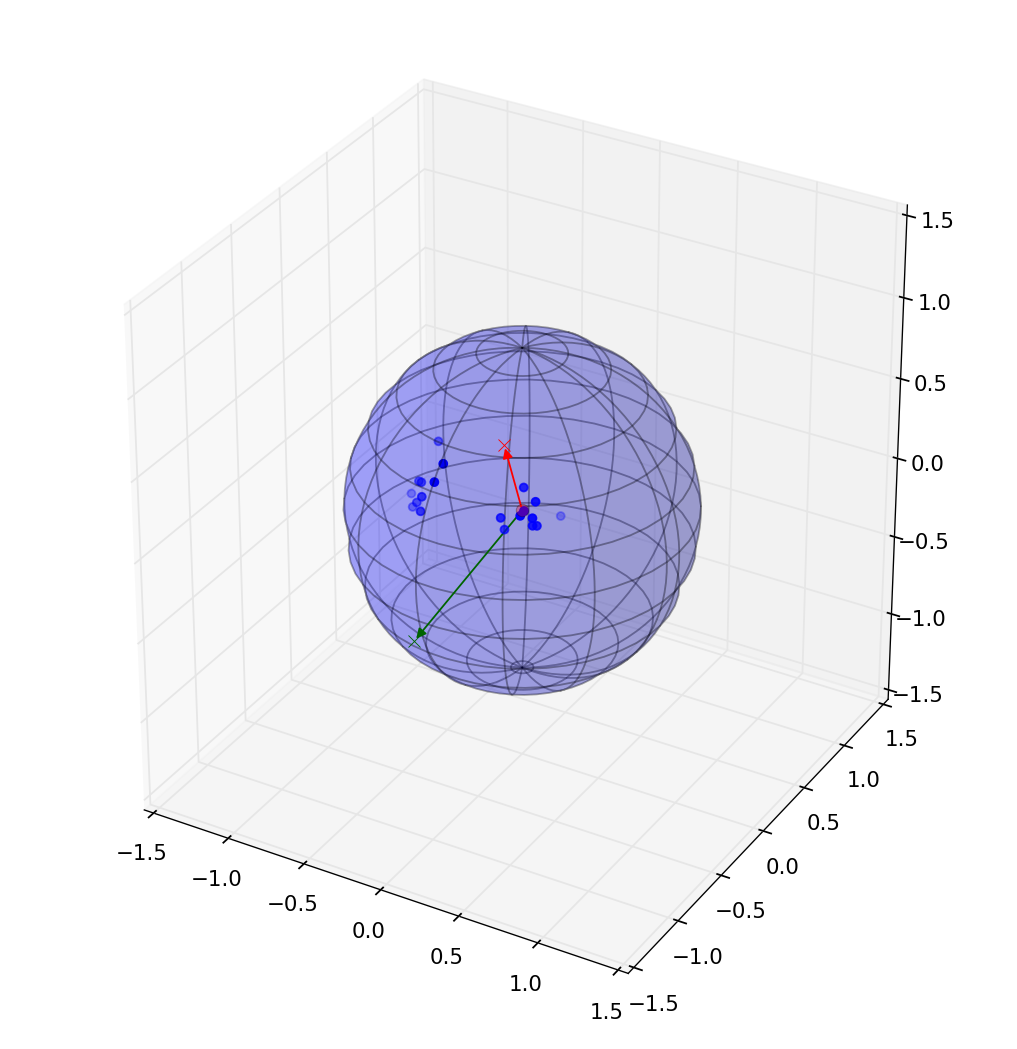
\includegraphics[width=0.75\textwidth, height=0.75\textwidth]{dead_unit.png}
        \end{center} }}
	\caption{An example of dead unit problem. Red and Green arrows are initialised weight before applying into the network. Green arrow is set far from both two input clusters, and it is assumed as a dead unit. Unfortunately, green arrow will never fire through the learning, and which means that input vectors are not properly clustered.}
	\label{fig:dead_unit}
\end{figure}

\begin{figure}[ht]
    \centering
    \framebox{\parbox[t][0.7\textwidth][t]{0.95\textwidth}{
        \begin{center}
            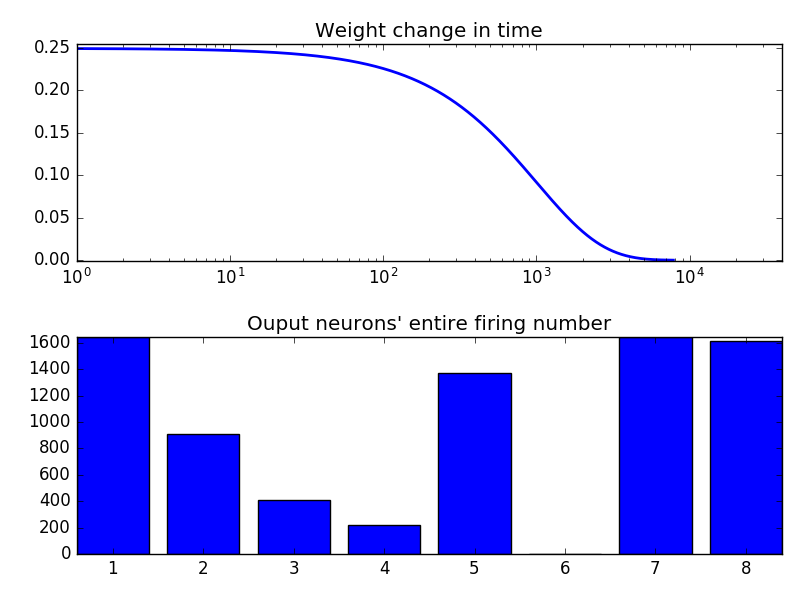
\includegraphics[width=0.85\textwidth, height=0.65\textwidth]{dead_state.png}
        \end{center} }}
	\caption{Learning rate and existence of dead units}
	\label{fig:dead_state}
\end{figure}

In (\ref{fig:dead_state}), ??? never fired and it is the dead unit, even though neuron ?? and ?? won several time compared to other ?? output neurons.

\bigskip
There are several approaches which can tackle the dead units problem, and 4 of those;
\begin{enumerate}
    \item leaky learning (LL),
    \item add bias (AB),
    \item add noise (AN),
    \item initialisation within input space (SV),
\end{enumerate}
will be discussed.

\bigskip
First, leaky learning (LL) is the way of adjusting learning rate for both winner and lower output units. It gives loser units some chances to fire in the future, and they move towards more dense clusters. Equation of LL is as follow,
\begin{equation} \label{eq:leaky_learning}
\begin{split}
w_{ij}^{new} & = w_{ij}^{old} + \eta_{winner} (x_i - w_{ij}^{old}), \\
w_{ij}^{new} & = w_{ij}^{old} + \eta_{loser} (x_i - w_{ij}^{old}), \quad \text{where } \eta_{winner} \gg \eta_{loser} \, .
\end{split}
\end{equation}

\bigskip
The second way to deal with dead units is adding bias (AB) to winner output unis which repeatedly fire. Then, they become hard to win again and again. 
\begin{equation} \label{eq:add_bias}
\begin{split}
f_j^{new} & = f_j^{old} + \beta (z_j - f_j^{old}), \\
b_j & = \gamma (1/n - f_j), \\
w_{ij}^{new} & = w_{ij}^{old} + \alpha (x_i - w_{ij}^{old}) z_j,\\
y_j & = \Sigma_i w_{ij} x + b_j \, ,
\end{split}
\end{equation}
where $z_j$ is a selector with a value of 0 for loser or 1 for winner, $\gamma, \beta$ are constant factors, $n$ is total nodes, $f$ is firing rate of output neuron, and $b$ is bias. By varying these parameters in (\ref{eq:add_bias}), learning performance can be adjusted.

\bigskip
Next is to add noise (AN) to output neurons while they are being updated. For the on-line game data analysis, Gaussian distribution are added to all output neurons. Then, among the output units with Gaussian noises, the largest output neuron is taken as a winner unit. Because of randomness, it is possible that frequently winner neurons may not fire even in the situations when the winner and loser output units are obvious from the equation (\ref{eq:distance}).
\begin{equation} \label{eq:add_noise}
\begin{split}
y_j & = \Sigma_{i}w_{ij}x_i + \epsilon, \\
& where \,\, \epsilon \sim N(0, \sigma^2)
\end{split}
\end{equation}
This is the simplest method to escape dead units problem, by just adding noises to outputs, one of loser units may take the place to win, instead of actual winner output neuron.

\bigskip
The last approach is to initialise weight vectors with randomly sampled vectors from input space. Three approaches which are discussed above do not solve the fundamental problem of dead units, and they still have the risk that some weight vectors are set far from any cluster. Because they randomly initialise weight vectors.

However, SV set initial weights in the actual input space. Therefore, they are always positioned inside the data set. Although they may manage dead units, there is other problem that some weight vectors are initialised near to each other. If some weight vectors are set nearly, they will converge the same optima, and data set will not properly clustered. 

Thus, large (LSD) or small(SSD) values randomly sampled with Gaussian distribution are added to the initial weight vectors, so that they have enough distance from each other.

\begin{equation} \label{eq9}
\begin{split}
w_{ij}^{init} & = w_{ij}^{random} + \epsilon, \\
& where \,\, \epsilon \sim N(0, \sigma^2)
\end{split}
\end{equation}

\begin{figure}[t]
    \centering
    \framebox{\parbox[t][0.7\textwidth][t]{0.95\textwidth}{
        \begin{center}
            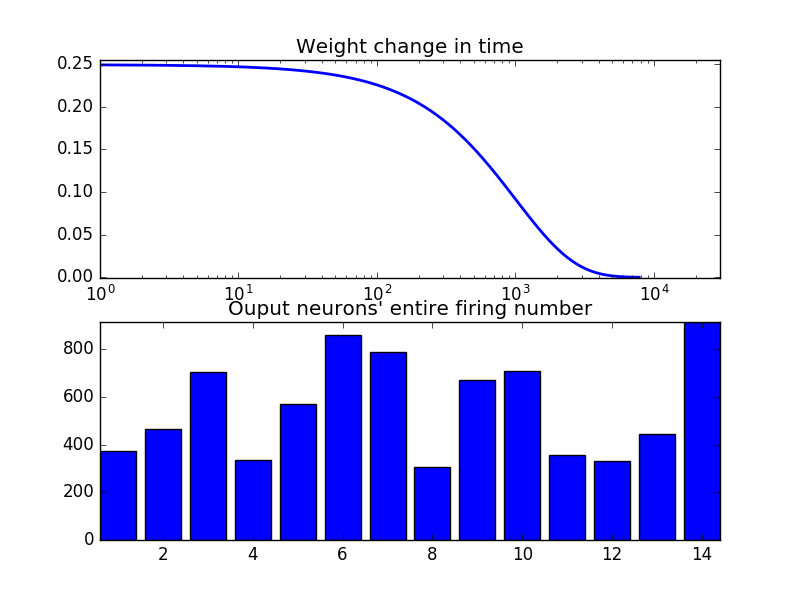
\includegraphics[width=0.85\textwidth, height=0.65\textwidth]{dead_states_solved.png}
        \end{center} }}
	\caption{Learning rate and and entire firing number of output neurons after using SV approach for dead units}
    \label{fig:dead_states_solved}
\end{figure}

\bigskip
In (\ref{fig:dead_states_solved}), it is shown that dead units are not exist. All output neurons fired above about 300 times, though some clusters are dominant in learning. This also give assumptions of how many individuals are belong to each cluster. It has to be noted that output firing state only give a rough estimate, as competitive algorithm exploit random point choice to compare with centroids. In addition, because there are no labelled and predefined features in the data set, there is no way to know how correct a result of clustering is. Thus, the data set is considered as unbiased, which means average from 10 iterations may represent the true value of the population.

% ======================================= %
%		2.4.5 Result
% ======================================= %
\newpage
\subsection{Centroids}

In conclusion of data curation, 1,201,516 individuals are grouped into 14 clusters as Fig.\ref{fig:centroid1}, \ref{fig:centroid2}, \ref{fig:centroid3}. Note that these are the results of truncated 15 attempts. 

\begin{figure}[h]
    \centering
    \framebox{\parbox[t][0.35\textheight][t]{0.95\textwidth}{
        \begin{center}
            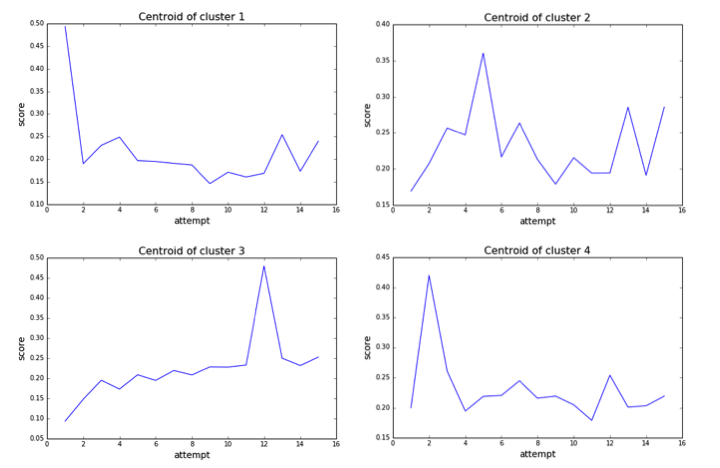
\includegraphics[width=0.9\textwidth, height=0.3\textheight]{centroid1.png}
        \end{center} }}
	\caption{Centroids of cluster from 1 to 4}
    \label{fig:centroid1}
\end{figure}

\begin{figure}[hb]
    \centering
    \framebox{\parbox[t][0.35\textheight][t]{0.95\textwidth}{
        \begin{center}
            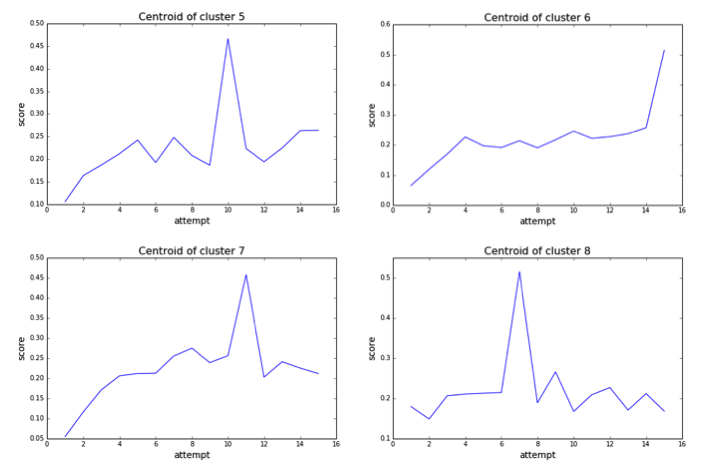
\includegraphics[width=0.9\textwidth, height=0.3\textheight]{centroid2.png}
        \end{center} }}
	\caption{Centroids of cluster from 5 to 8}
    \label{fig:centroid2}
\end{figure}

\begin{figure}[hb]
    \centering
    \framebox{\parbox[t][0.35\textheight][t]{0.95\textwidth}{
        \begin{center}
            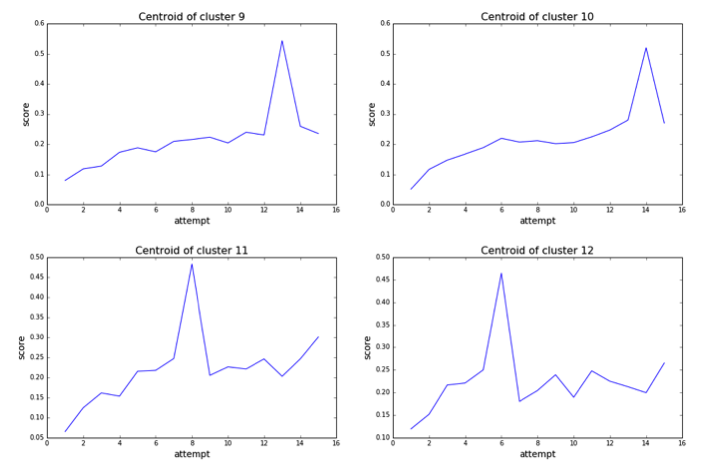
\includegraphics[width=0.9\textwidth, height=0.3\textheight]{centroid3.png}
        \end{center} }}
	\caption{Centroids of cluster from 9 to 12}
    \label{fig:centroid3}
\end{figure}

\begin{figure}[t]
    \centering
    \framebox{\parbox[t][0.23\textheight][t]{0.95\textwidth}{
        \begin{center}
            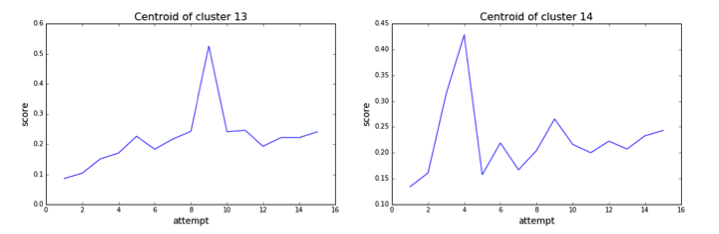
\includegraphics[width=0.9\textwidth, height=0.2\textheight]{centroid4.png}
        \end{center} }}
	\caption{Centroids of cluster 13 and 14}
    \label{fig:centroid4}
\end{figure}

In the next chapter, various curves are fitted to these centroids, and which curve can properly represent learning process for each group.

% ======================================================== %
%		2. Data Curation
% ======================================================== %
\chapter{Function Fitting}

%%%%%%%%%%% HINT %%%%%%%%%%%%%%%%%%%%%%%%%%%%%
% Ideally, you should generate a bibtex file (references.bib) and include all
% references in the bibtex format into this file. The reference list
% can then be automatically generated using bibtex.
%%%%%%%%%%%%%%%%%%%%%%%%%%%%%%%%%%%%%%%%%%%%

\begin{comment}
\begin{thebibliography}{20}

\addcontentsline{toc}{chapter}{REFERENCES}

%\bibitem{test} 
% \bibitem{lowry1951protein}Lowry, O. H., Rosebrough, N. J., Farr, A. L., and Randall, R. J. (1951). Protein measurement with the Folin phenol reagent. \emph{J. Biol. Chem.}, 193(1), 265--275.

\bibitem{Idris 2014} Idris, I. (2014). \emph{Python Data Analysis}. Packt Publishing Ltd.

\bibitem{Python 2001} Python(TM). (2001). \emph{12.1. Pickle - python object serialization - python 3.5.2 documentation}. Retrieved June 30, 2016, from Python 3.5.2 Document, https://docs.python.org/3/library/pickle.html\#data-stream-format

\bibitem{Shafranovich 2008} Shafranovich, Y. (2008). Common Format and MIME Type for Comma-Separated Values (CSV) Files.[Sl], 2005. \emph{Dispon?vel em:$<$ http://www. ietf. org/rfc/rfc4180. txt.}

\bibitem{Stuart 2012} P. Stuart, "Axon - a game for science," 2012. [Online]. Available: http://preloaded.com/axon-game-science/. Accessed: Jun. 24, 2016.

\bibitem{Stafford et al. 2014} Stafford, T., \& Dewar, M. (2014). Tracing the trajectory of skill learning with a very large sample of online game players. \emph{Psychological Science}, 25(2), 511-518.

\bibitem{Stafford et al. 2016} Stafford, T., \& Haasnoot, E. (2016). Testing sleep consolidation in skill learning: a field study using an online game. \emph{Topics in Cognitive Science}.

\bibitem{Stonebraker et al. 2013} Stonebraker, M., Bruckner, D., Ilyas, I. F., Beskales, G., Cherniack, M., Zdonik, S. B.,  Alexander, P., \& Xu, S. (2013, January). Data Curation at Scale: The Data Tamer System. In \emph{CIDR}.

\bibitem{Gallistel et al. 2004} Gallistel, C. R., Fairhurst, S., \& Balsam, P. (2004). The learning curve: Implications of a quantitative analysis. \emph{Proceedings of the National Academy of Sciences, 101}(36), pp.13124?13131.

\bibitem{Newell 1981} Newell, A., \& Rosenbloom, P. S. (1981). Mechanisms of skill acquisition and the law of practice. \emph{Cognitive skills and their acquisition, 1}, pp. 1-55.

\bibitem{Donner 2015} Donner, Y., \& Hardy, J. L. (2015). Piecewise power laws in individual learning curves. \emph{Psychonomic Bulletin \& Review, 22}(5), pp. 1308?1319.

\bibitem{Gaschler et al. 2014} Gaschler, R., Progscha, J., Smallbone, K., Ram, N., \& Bilalic, M. (2014). Playing off the curve -testing quantitative predictions of skill acquisition theories in development of chess performance. \emph{Frontiers in Psychology, 5}, pp. 1?11.

\bibitem{Howard 2014} Howard, R. W. (2014). Learning curves in highly skilled chess players: A test of the generality of the power law of practice. \emph{Acta Psychologica, 151}, pp. 16?23. 

\bibitem{Heathcote et al. 2000} Heathcote, a, Brown, S., \& Mewhort, D. J. (2000). The power law repealed: the case for an exponential law of practice. \emph{Psychonomic Bulletin \& Review, 7}(2), pp. 185?207.

\bibitem{Murre 2011} Murre, J. M., \& Chessa, A. G. (2011). Power laws from individual differences in learning and forgetting: mathematical analyses. \emph{Psychonomic bulletin \& review, 18}(3), pp. 592-597.

\bibitem{Hackeling 2014} Hackeling, G. (2014). \emph{Mastering Machine Learning with scikit-learn}. Packt Publishing Ltd.

\bibitem{Harrington 2012} Harrington, P. (2012). \emph{Machine learning in action} (Vol. 5). Greenwich, CT: Manning.

\bibitem{Daume III 2012} Daume III, H. (2012). \emph{A course in Machine Learning}: ciml.info

\bibitem{Michael 2015} Michael, B. 2015 \emph{Machine Learning in Python: Essential Techniques for Predictive Analysis}. Indianapolis: John Wiley \& Sons, Inc.

\end{thebibliography}
\end{comment}

\nocite{*}
\bibliographystyle{apacite}
%\bibliographystyle{apalike}
\bibliography{references}
\end{document}

%\begin{gather*} 
%2x - 5y =  8 \\ 
%3x^2 + 9y =  3a + c
%\end{gather*}
